\documentclass[handout, 11pt]{beamer}
\mode
<presentation>{\usetheme{Madrid}}
\institute[UF]{\inst{1}
University of Florida\\
Department of Finance, Insurance, and Real Estate}
\usepackage{adjustbox}
\usepackage{tikz}
\usetikzlibrary{positioning}
\usetikzlibrary{positioning}
\usetikzlibrary{positioning}
\usetikzlibrary{positioning}
\usetikzlibrary{positioning}
\usetikzlibrary{positioning}
\usetikzlibrary{positioning}
\usetikzlibrary{positioning}
\usetikzlibrary{positioning}
\usetikzlibrary{positioning}
\usetikzlibrary{positioning}
\usepackage{booktabs}
\definecolor{darkgreen}{RGB}{31,156,17}
\usepackage{xcolor}
\setbeamertemplate{headline}{\begin{beamercolorbox}[ht=2.25ex, dp=3.75ex]{section in head/foot}
\insertnavigation{\paperwidth}
\end{beamercolorbox}}
\AtBeginSection{\begin{frame}
\frametitle{Table of Contents}
\tableofcontents[currentsection]
\end{frame}}
\begin{document}
\title[Intro DCF and Cost of Capital]{Introduction to DCF Valuation and Cost of Capital Estimation}
\subtitle{A Primer on DCF Valuation and Exploring the Cost of Capital Section of the Model}
\author[DeRobertis]{Nick DeRobertis\inst{1}}
\date{\today}
\begin{frame}
\titlepage
\label{title-frame}
\end{frame}
\begin{section}[DCF Intro]{Introduction to Discounted Cash Flow (DCF) Valuation}
\begin{frame}
\frametitle{What is a DCF?}
\begin{itemize}
\item A \textbf{discounted cash flow valuation (DCF)} is a method of determining the value of a stock.
\vfill
\item Other ways include the dividend discount model and approaches based on comparables
\vfill
\item The dividend discount model only works well for stable companies that pay dividends with constant growth.
\vfill
\item Comparable approaches can give a rough idea of a valuation but never take into account the specifics of the company
\vfill
\item DCF valuation can be applied to any company and is based on the particulars of the company
\end{itemize}
\end{frame}
\begin{frame}
\frametitle{The DCF in One Picture}
\begin{center}
\begin{adjustbox}{width=0.9\textwidth, height=0.8\textheight, keepaspectratio}
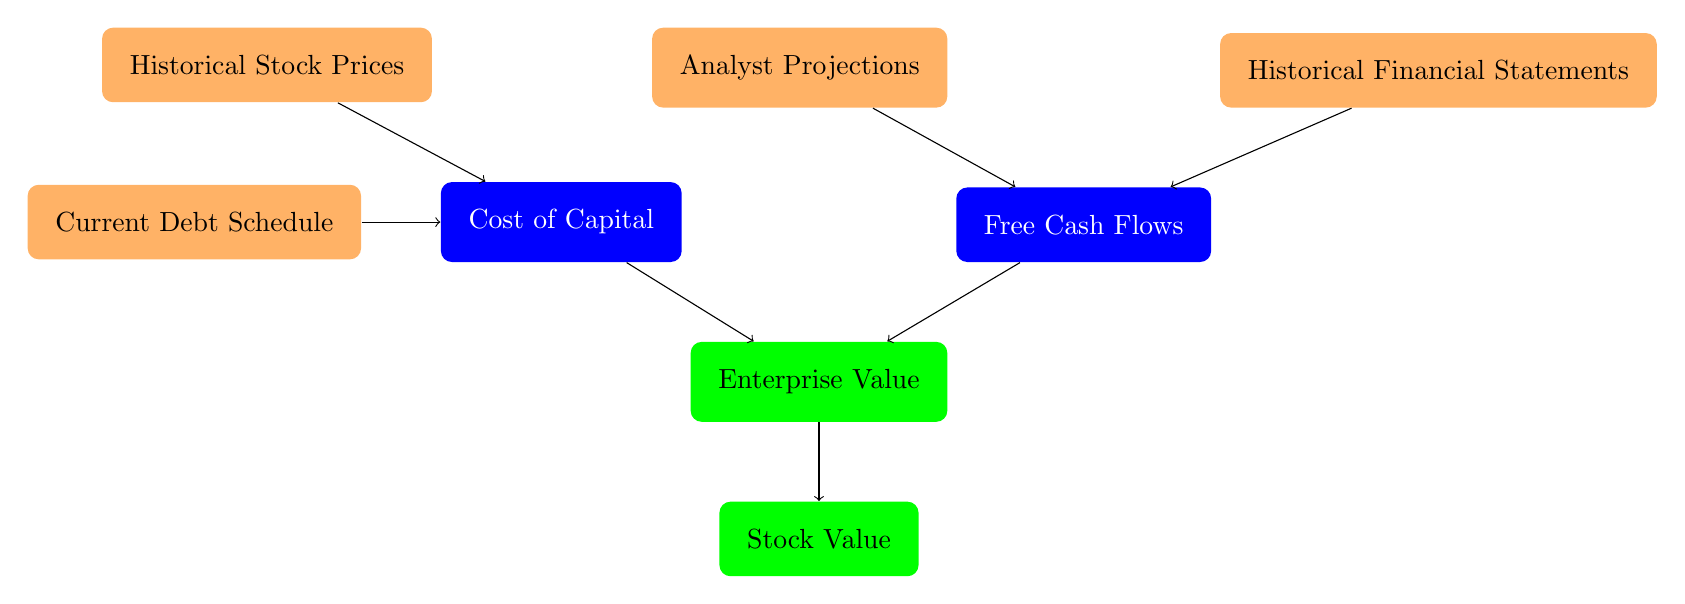
\begin{tikzpicture}
\node [inner sep=10pt, rounded corners, fill=green] (c76dabc2-1964-4a10-b72a-88fafa6f2138)  {Stock Value};
\node [inner sep=10pt, rounded corners, fill=green, above=of c76dabc2-1964-4a10-b72a-88fafa6f2138] (ab3d5dad-7dfb-43ae-aa5d-3acc752e0aad)  {Enterprise Value};
\node [inner sep=10pt, rounded corners, fill=blue, text=white, above right=and 0.1cm of ab3d5dad-7dfb-43ae-aa5d-3acc752e0aad] (f9bf7c24-76fd-46b5-aab1-e33305c3d589)  {Free Cash Flows};
\node [inner sep=10pt, rounded corners, fill=orange!60, above right=and 0.1cm of f9bf7c24-76fd-46b5-aab1-e33305c3d589] (77b7cfc5-f237-4b8b-ade6-b2b41b402949)  {Historical Financial Statements};
\node [inner sep=10pt, rounded corners, fill=orange!60, above left=and 0.1cm of f9bf7c24-76fd-46b5-aab1-e33305c3d589] (170050d0-04a2-4a41-8a84-c7c58c1e31e8)  {Analyst Projections};
\node [inner sep=10pt, rounded corners, fill=blue, text=white, above left=and 0.1cm of ab3d5dad-7dfb-43ae-aa5d-3acc752e0aad] (4a6151fc-a83a-4b5b-9e7c-e5ffde1e4b60)  {Cost of Capital};
\node [inner sep=10pt, rounded corners, fill=orange!60, left=of 4a6151fc-a83a-4b5b-9e7c-e5ffde1e4b60] (755d7c98-4778-44f2-bbf4-030d2473a6b6)  {Current Debt Schedule};
\node [inner sep=10pt, rounded corners, fill=orange!60, above left=and 0.1cm of 4a6151fc-a83a-4b5b-9e7c-e5ffde1e4b60] (133a4ad1-cb06-49dc-9e20-34fbe122a1bf)  {Historical Stock Prices};
\path [draw, ->] (ab3d5dad-7dfb-43ae-aa5d-3acc752e0aad) -- (c76dabc2-1964-4a10-b72a-88fafa6f2138);
\path [draw, ->] (f9bf7c24-76fd-46b5-aab1-e33305c3d589) -- (ab3d5dad-7dfb-43ae-aa5d-3acc752e0aad);
\path [draw, ->] (77b7cfc5-f237-4b8b-ade6-b2b41b402949) -- (f9bf7c24-76fd-46b5-aab1-e33305c3d589);
\path [draw, ->] (170050d0-04a2-4a41-8a84-c7c58c1e31e8) -- (f9bf7c24-76fd-46b5-aab1-e33305c3d589);
\path [draw, ->] (4a6151fc-a83a-4b5b-9e7c-e5ffde1e4b60) -- (ab3d5dad-7dfb-43ae-aa5d-3acc752e0aad);
\path [draw, ->] (755d7c98-4778-44f2-bbf4-030d2473a6b6) -- (4a6151fc-a83a-4b5b-9e7c-e5ffde1e4b60);
\path [draw, ->] (133a4ad1-cb06-49dc-9e20-34fbe122a1bf) -- (4a6151fc-a83a-4b5b-9e7c-e5ffde1e4b60);
\end{tikzpicture}
\end{adjustbox}
\end{center}
\end{frame}
\begin{frame}
\frametitle{Motivating the DCF}
\begin{block}{Financial Asset Value}
\begin{equation}
	V = \sum_{t=0}^T \frac{CF^t}{(1 + r)^t}
\end{equation}
\end{block}
\begin{itemize}
\item The value of any financial asset is the present value of its future cash flows
\vfill
\item The cash flows for a stock are dividends. The dividend discount model takes the present value of future dividends.
\vfill
\item To find the value of a business, find the present value of its future free cash flows
\end{itemize}
\end{frame}
\begin{frame}
\frametitle{Overview of Cost of Capital Estimation}
\begin{columns}
\begin{column}{0.5\textwidth}
\vbox to 0.8\textheight{\begin{itemize}
\small
\vfill
\item The goal of cost of capital estimation is to determine the
\textbf{weighted average cost of capital (WACC)}
\vfill
\item This can broadly be broken down into two components: estimating the
\underline{cost of equity}
and estimating the
\underline{cost of debt}
\vfill
\item Cost of equity is typically estimated using the Capital Asset Pricing Model (CAPM)
\vfill
\item Cost of debt is usually estimated from the interest payments and book value of debt
\end{itemize}}
\end{column}
\begin{column}{0.5\textwidth}
\vbox to 0.8\textheight{\centering
\vfill
\begin{center}
\begin{adjustbox}{width=0.9\textwidth, height=0.8\textheight, keepaspectratio}
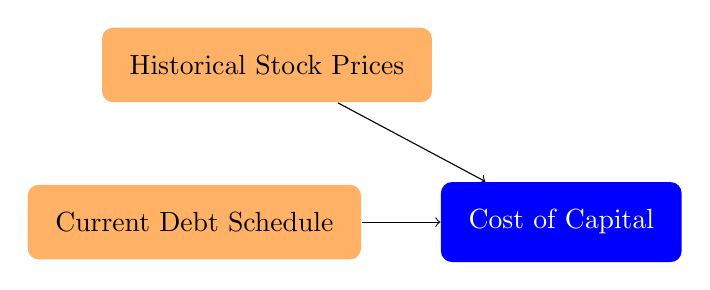
\begin{tikzpicture}
\node [inner sep=10pt, rounded corners, fill=blue, text=white] (80db54e7-5856-4ac2-83b1-7aaf33e6df66)  {Cost of Capital};
\node [inner sep=10pt, rounded corners, fill=orange!60, left=of 80db54e7-5856-4ac2-83b1-7aaf33e6df66] (c112de39-eed3-4d4d-a44c-c4ed6acd5201)  {Current Debt Schedule};
\node [inner sep=10pt, rounded corners, fill=orange!60, above left=and 0.1cm of 80db54e7-5856-4ac2-83b1-7aaf33e6df66] (8fe197b4-2a19-4c68-b29d-77606584eb06)  {Historical Stock Prices};
\path [draw, ->] (c112de39-eed3-4d4d-a44c-c4ed6acd5201) -- (80db54e7-5856-4ac2-83b1-7aaf33e6df66);
\path [draw, ->] (8fe197b4-2a19-4c68-b29d-77606584eb06) -- (80db54e7-5856-4ac2-83b1-7aaf33e6df66);
\end{tikzpicture}
\end{adjustbox}
\end{center}
\vfill
\vfill}
\end{column}
\end{columns}
\end{frame}
\begin{frame}
\frametitle{Overview of Free Cash Flow Estimation}
\begin{columns}
\begin{column}{0.5\textwidth}
\vbox to 0.8\textheight{\begin{itemize}
\small
\vfill
\item The goal of free cash flow estimation is to determine the historical and future free cash flows (FCF) for the company.
\vfill
\item Historical financial statements, including the income statement, balance sheet, and statement of cash flows are used to determine historical FCF
\vfill
\item It is the job of the analyst building the model to project those FCF into the future
\vfill
\item This is usually done by projecting the financial statements into the future
\end{itemize}}
\end{column}
\begin{column}{0.5\textwidth}
\vbox to 0.8\textheight{\centering
\vfill
\begin{center}
\begin{adjustbox}{width=0.9\textwidth, height=0.8\textheight, keepaspectratio}
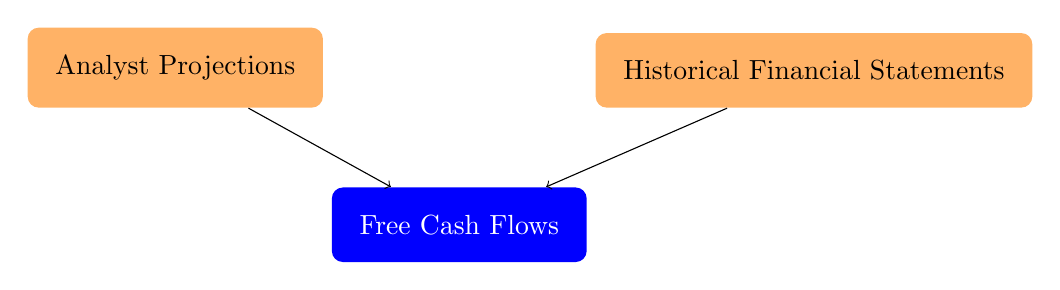
\begin{tikzpicture}
\node [inner sep=10pt, rounded corners, fill=blue, text=white] (fc4cf0e5-0c0b-4c33-b31a-5733e1241913)  {Free Cash Flows};
\node [inner sep=10pt, rounded corners, fill=orange!60, above right=and 0.1cm of fc4cf0e5-0c0b-4c33-b31a-5733e1241913] (228c44fd-358e-471a-ba35-a10d2827c4bf)  {Historical Financial Statements};
\node [inner sep=10pt, rounded corners, fill=orange!60, above left=and 0.1cm of fc4cf0e5-0c0b-4c33-b31a-5733e1241913] (ec5d97db-2b15-4d47-b739-37459c049e05)  {Analyst Projections};
\path [draw, ->] (228c44fd-358e-471a-ba35-a10d2827c4bf) -- (fc4cf0e5-0c0b-4c33-b31a-5733e1241913);
\path [draw, ->] (ec5d97db-2b15-4d47-b739-37459c049e05) -- (fc4cf0e5-0c0b-4c33-b31a-5733e1241913);
\end{tikzpicture}
\end{adjustbox}
\end{center}
\vfill
\vfill}
\end{column}
\end{columns}
\end{frame}
\end{section}
\begin{section}[EV]{Enterprise and Equity Value}
\begin{frame}
\frametitle{Enterprise Value vs. Equity Value}
\begin{itemize}
\item The enterprise value of the business is the asset value or the cost to purchase the entire company
\vfill
\item $\text{Enterprise Value} = \text{Equity Value} + \text{Debt Value} - \text{Cash}$
\vfill
\item A stock represents only the equity value or market capitalization of a business
\vfill
\item By determining the enterprise value, we can back into the equity value to get the stock price
\end{itemize}
\end{frame}
\small
\begin{frame}
\frametitle{Enterprise and Equity Value Lab, Level 1}
{
\setbeamercolor{block title}{bg=violet}
\begin{block}{Finding Enterprise and Equity Value Given FCF and WACC, Level 1}
\begin{enumerate}
\item You are the CFO for a startup developing artificial intelligence technologies. There will be an initial research phase before making any money. Google is watching your development and will purchase the company after it is profitable.
\item For the first two years (years 0 and 1), the company loses \$20 million. Then there is one breakeven year, after which the profit is \$10 million for year 3. Finally in year 4, Google purchases the company for \$70 million.
\item The WACC for the company is 15\% and it has 1 million shares outstanding. The company has \$5 million in debt and \$1 million in cash.
\item What is the enterprise value of the stock at year 5? What about the enterprise value today? What is the price of the stock today?
\end{enumerate}
\vfill
\begin{tabular*}{\textwidth}{@{\extracolsep{\fill}}ccccc}
\toprule
\hfill & Level 2: Slide \textcolor{blue}{\underline{\ref{labs:enterprise-and-equity-value-lab-2}}} & Answers 1: Slide \textcolor{blue}{\underline{\ref{labs:enterprise-and-equity-value-lab-1-answers}}} & Resources: Slide \textcolor{blue}{\underline{\ref{labs:enterprise-and-equity-value-lab-1-resources}}} & \hfill\\

\end{tabular*}
\end{block}
}
\label{labs:enterprise-and-equity-value-lab-1}
\end{frame}
\normalsize
\end{section}
\begin{section}[Equity]{Cost of Equity Estimation}
\begin{frame}
\frametitle{How Can CAPM be used for Estimating the Cost of Equity?}
\small
\begin{block}{Capital Asset Pricing Model (CAPM)}
\begin{equation}
	r_i = r_f + \beta (r_m - r_f) + \epsilon
\end{equation}
\vspace{-0.3cm}
\begin{itemize}
\item $r_i$: Return on stock $i$
\item $r_f$: Return on risk free asset
\item $r_m$: Return on market portfolio
\item $\beta$: Covariance of stock returns with market risk premium
\item $\epsilon$: Idiosyncratic return, mean 0
\end{itemize}
\end{block}
\begin{itemize}
\item We will use historical stock price data along with CAPM to produce an estimate of the cost of equity.
\vfill
\item Ultimately, $r_i$ is the estimate of the cost of equity
\end{itemize}
\end{frame}
\begin{frame}
\frametitle{Overview of Cost of Equity Estimation}
\begin{block}{Capital Asset Pricing Model (CAPM)}
$r_i = r_f + \beta (r_m - r_f) + \epsilon$
\end{block}
\begin{itemize}
\item The three returns can all be estimated from historical data. Therefore $\beta$ and $\epsilon$ are the unknowns. But $\epsilon$ has mean zero so we can ignore it for estimation.
\vfill
\item We will estimate the historical beta, then assume that the beta is still valid today to come up with the current $r_i$ as the cost of equity.
\vfill
\item $\beta$ can be estimated by regressing the historical stock returns of the company on the historical market risk premiums. The $\beta$ is then the coefficient of the market risk premium in the regression.
\end{itemize}
\end{frame}
\begin{frame}
\frametitle{Using Price Data to Estimate Cost of Equity in Python}
{
\setbeamercolor{block title}{bg=darkgreen}
\begin{block}{Python CAPM Estimation}
\begin{itemize}
\item Go to Canvas and download "Determining the Cost of Equity.ipynb" and "price data.xlsx" from Examples > DCF > Cost of Equity > Python
\item Make sure that you place these two in the same folder
\item We are using historical prices to calculate the cost of equity using CAPM
\item We will use a risk free rate of 3\% for the exercise
\end{itemize}
\end{block}
}
\end{frame}
\begin{frame}
\frametitle{Using Price Data to Estimate Cost of Equity in Excel}
{
\setbeamercolor{block title}{bg=darkgreen}
\begin{block}{Excel CAPM Estimation}
\begin{itemize}
\item Go to Canvas and download "DCF Cost of Equity.xlsx" from Examples > DCF > Cost of Equity > Excel
\item We are using historical prices to calculate the cost of equity using CAPM
\item We will use a risk free rate of 3\% for the exercise
\end{itemize}
\end{block}
}
\end{frame}
\begin{frame}
\frametitle{DCF Cost of Equity Lab}
{
\setbeamercolor{block title}{bg=violet}
\begin{block}{Finding Cost of Equity Given Historical Prices}
\begin{enumerate}
\item Download "prices.xlsx" from the course site
\item Assume the risk free rate is 2\%
\item What is the beta and the cost of equity for this company?
\item If you thought there was going to be a recession, such that the average market return would be 3\% lower, then what would you expect the cost of equity to be?
\item Complete this exercise with the tool of your choice.
\end{enumerate}
\vfill
\begin{tabular*}{\textwidth}{@{\extracolsep{\fill}}cccc}
\toprule
\hfill & Answers: Slide \textcolor{blue}{\underline{\ref{labs:dcf-cost-of-equity-lab-1-answers}}} & Resources: Slide \textcolor{blue}{\underline{\ref{labs:dcf-cost-of-equity-lab-1-resources}}} & \hfill\\

\end{tabular*}
\end{block}
}
\label{labs:dcf-cost-of-equity-lab-1}
\end{frame}
\begin{frame}
\frametitle{Market Value of Equity}
\begin{itemize}
\item As we will cover in more detail when we get to WACC, we need to have the market values of both equity and debt along with the costs to be able to caluclate the WACC.
\vfill
\item The market value of equity for a publicly traded company is straightforward. Just calculate the \textbf{market capitalization} as the number of shares outstanding multiplied by the current share price.
\vfill
\item The market capitalization can be used directly as the market value of equity.
\end{itemize}
\end{frame}
\end{section}
\begin{section}[Debt]{Cost of Debt Estimation}
\begin{frame}
\frametitle{Overview of Estimating the Cost of Debt}
\begin{itemize}
\item We want to estimate the cost of debt for the company, which more specifically should be the marginal interest cost of raising one additional dollar via debt.
\vfill
\item There are two general approaches to estimating this: the
\underline{financial statements approach}
and the
\underline{market value of bonds approach}
\vfill
\item The market value of bonds approach is better able to capture the current rate when it has changed substantially over time, but it requires price, coupon, and maturity information on a bond.
\vfill
\item The financial statements approach uses only the income statement and balance sheet, and represents a weighted average historical cost of debt.
\end{itemize}
\end{frame}
\begin{frame}
\frametitle{The Financial Statements Approach to Cost of Debt}
\begin{itemize}
\item The financial statements approach uses interest expense from the income statement and total debt from the balance sheet to estimate the cost of debt
\vfill
\item With this approach, we can estimate the cost of debt by a very simple formula
\vfill
\item $r_d = \frac{\text{Interest Expense}}{\text{Total Debt}}$
\vfill
\item Calculate this for the most recent data available and use this as the cost of debt
\end{itemize}
\end{frame}
\begin{frame}
\frametitle{The Market Value of Bonds Approach to Cost of Debt}
\begin{itemize}
\item The cost of debt is about raising new debt, so it is more accurate to look at the market to determine how much the company would have to pay for new debt.
\vfill
\item The yield to maturity (YTM) of the company's bonds can be calculated. A weighted average of the YTMs can be used as an estimate of the cost of debt.
\vfill
\item The YTM is representing the required rate of return on the bond for the investor, which is equivalent to the cost of the bond for the company
\vfill
\item The YTM is simply the IRR of the bond, considering the current market price of the bond
\end{itemize}
\end{frame}
\begin{frame}
\frametitle{After-Tax Cost of Debt}
\begin{itemize}
\small
\vfill
\item Debt has an interesting feature in our tax system: debt is
\underline{tax deductible.}
\vfill
\item The amount a company has to pay in income tax is taken as a percentage of earnings before tax (EBT).
\vfill
\item As interest is taken out while calculating EBT, it lowers the tax payment.
\vfill
\item Think about two hypothetical companies with the exact same operations, revenues, costs, etc. One is financed completely with equity and the other with 50\% debt. They will both have the same EBIT but the EBT will be lower for the debt firm and so the taxes will be lower for the debt firm, likely giving the debt firm a higher value than the equity firm.
\vfill
\item What this means for cost of capital estimation is that all our calculations will be based on pre-tax numbers, then we multiply by $(1 - \text{tax rate})$ to get the after-tax cost of debt to use in the WACC.
\end{itemize}
\end{frame}
\begin{frame}
\frametitle{DCF Cost of Debt Lab, Level 1}
{
\setbeamercolor{block title}{bg=violet}
\begin{block}{Finding Cost of Debt Given Financial and Market Info, Level 1}
\begin{enumerate}
\item A chemical manufacturer has a 7.0\% coupon, annual pay 1000 par value bond outstanding, priced at \$1042.12 on 2020-10-07.
\item If the bond matures on 2023-10-07, what is the cost of debt for this company? The tax rate is 35\%.
\end{enumerate}
\vfill
\begin{tabular*}{\textwidth}{@{\extracolsep{\fill}}ccccc}
\toprule
\hfill & Level 2: Slide \textcolor{blue}{\underline{\ref{labs:dcf-cost-of-debt-lab-2}}} & Answers 1: Slide \textcolor{blue}{\underline{\ref{labs:dcf-cost-of-debt-lab-1-answers}}} & Resources: Slide \textcolor{blue}{\underline{\ref{labs:dcf-cost-of-debt-lab-1-resources}}} & \hfill\\

\end{tabular*}
\end{block}
}
\label{labs:dcf-cost-of-debt-lab-1}
\end{frame}
\begin{frame}
\frametitle{What is the Market Value of Debt?}
\begin{itemize}
\item If you have taken the debt course, you should be familiar with the fact that bonds' values change over time.
\vfill
\item The value of a bond can be determined (just like any financial asset) by taking the present value of future cash flows (here, interest and principal payments). 
\vfill
\item If the discount rate for the company changes, the value of the bonds change, as the interest payments are contracted and will remain the same
\vfill
\item The discount rate will change when the riskiness of the firm's debt changes, e.g. taking on additional debt, starting a new project, having a bad operating year, etc.
\end{itemize}
\end{frame}
\begin{frame}
\frametitle{Why Should we Care about the Market Value of Debt?}
\begin{itemize}
\item Say a company issues a 3-year bond with a 10\% coupon. When issued, the riskiness of the firm implies it should have a 10\% discount rate. In other words, the true cost of debt is 10\%. The bond is at par (value 1,000).
\vfill
\item One year later, the firm has a bad year, and now lenders are requiring a 15\% rate to lend to the company
\vfill
\item Due to this, the price of the existing bond has dropped to \$918.71.
\vfill
\item If we calculate the IRR on this \$918.71 bond, it comes to 15\%, which is the true YTM or cost of debt
\vfill
\item The coupon rate on the bond is still 10\%, and the book value of debt on the balance sheet is still 1,000 so based on the financial statements approach the cost of debt would still be 10\%.
\end{itemize}
\end{frame}
\begin{frame}
\frametitle{Approaches to Calculating the Market Value of Debt}
\begin{itemize}
\item There are three main approaches to calculating the market value of debt for use in the WACC calculation, depending on what data you have available
\vfill
\item If all you have is financial statements, you must just
\underline{assume the book value of debt equals the market value of debt.}
\vfill
\item If you also have an estimate of the current cost of debt obtained from the market as well as an average maturity of debt, you can use the
\underline{hypothetical bond approach.}
\vfill
\item Finally, if you have all the individual debt instruments, you can
\underline{calculate the market value of individual instruments.}
\end{itemize}
\end{frame}
\begin{frame}
\frametitle{Calculating the Market Value of Debt}
{
\setbeamercolor{block title}{bg=darkgreen}
\begin{block}{MV Debt Example}
\begin{itemize}
\item Go to Canvas and download "Market Value of Debt.ipynb" and "debt data.xlsx" from Examples > DCF > Cost of Debt
\item Ensure you have the Jupyter notebook and the Excel spreadsheet in the same folder.
\item We will go through the Jupyter notebook to show the three approaches to estimating the market value of debt.
\end{itemize}
\end{block}
}
\end{frame}
\begin{frame}
\frametitle{Dealing with Seniority of Debt}
\begin{itemize}
\item For the purposes of this class, we won't deal with seniority. But you should keep it in mind in the future when estimating the market value of debt.
\vfill
\item Seniority represents the payoff order during bankruptcy. The most senior loans will be paid first, and if there is still money left over, then the more junior loans will be paid.
\vfill
\item As there is a higher expected value in recovery, senior loans are less risky and so should have a lower rate associated with them.
\vfill
\item In the prior exercise, when valuing individual debt instruments, we assumed a single cost of debt, when in reality, it should be adjusted for the seniority.
\end{itemize}
\end{frame}
\end{section}
\begin{section}[WACC]{Putting it All Together: Calculating the WACC}
\begin{frame}
\frametitle{Calculating WACC}
\begin{block}{Weighted Average Cost of Capital (WACC)}
\begin{equation}
	\text{WACC} = r_e w_e + r_d (1 - t) w_d
\end{equation}
\vspace{-0.4cm}
\begin{itemize}
\item $r_e$: Cost of equity
\item $w_e$: Weight of equity
\item $r_d$: Pre-tax cost of debt
\item $t$: Tax rate
\item $w_d$: Weight of debt
\end{itemize}
\end{block}
\begin{itemize}
\item So now from the prior sections we have the cost of equity, market value of equity, cost of debt, and market value of debt.
\vfill
\item The weights of debt and equity are found by dividing that market value by the sum of both market values.
\end{itemize}
\end{frame}
\begin{frame}
\frametitle{What the Weighted Part of WACC Means}
\begin{center}
\begin{adjustbox}{width=0.9\textwidth, height=0.35\textheight, keepaspectratio}
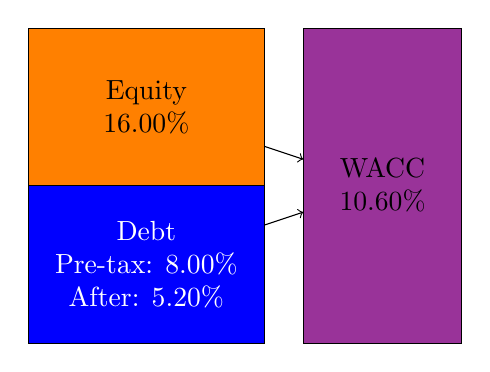
\begin{tikzpicture}
\node [every text node part/.style={align=center}, fill=blue, minimum width=3cm, minimum height=2.0cm, rectangle, draw, every text node part/.style={align=center}, text=white] (3cc024c3-c59c-4785-b03b-7a2ac843d684) at (0, 0) {Debt
\\
Pre-tax: 8.00\%
\\
After: 5.20\%};
\node [every text node part/.style={align=center}, fill=orange, minimum width=3cm, minimum height=2.0cm, rectangle, draw] (68b4c6ee-00a7-40d9-88fe-fb75febf9b0f) at (0, 2.0) {Equity
\\
16.00\%};
\node [every text node part/.style={align=center}, fill=violet!80, minimum width=2cm, minimum height=4cm, rectangle, draw] (e3ecad63-11ff-437b-bf47-b7a337066c1a) at (3, 1) {WACC
\\
10.60\%};
\path [draw, ->] (3cc024c3-c59c-4785-b03b-7a2ac843d684) -- (e3ecad63-11ff-437b-bf47-b7a337066c1a);
\path [draw, ->] (68b4c6ee-00a7-40d9-88fe-fb75febf9b0f) -- (e3ecad63-11ff-437b-bf47-b7a337066c1a);
\end{tikzpicture}
\end{adjustbox}
\end{center}
\begin{center}
\begin{adjustbox}{width=0.9\textwidth, height=0.35\textheight, keepaspectratio}
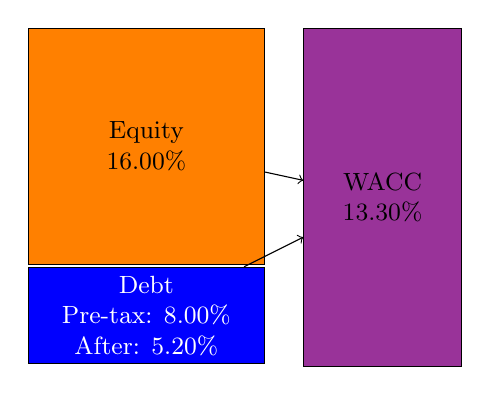
\begin{tikzpicture}
\small
\node [every text node part/.style={align=center}, fill=blue, minimum width=3cm, minimum height=1.0cm, rectangle, draw, every text node part/.style={align=center}, text=white] (dde1cb4a-3654-423a-9639-0239efc395c9) at (0, 0) {Debt
\\
Pre-tax: 8.00\%
\\
After: 5.20\%};
\node [every text node part/.style={align=center}, fill=orange, minimum width=3cm, minimum height=3.0cm, rectangle, draw] (bd9a2309-8b7f-4c79-a6df-f8a69e27b9b5) at (0, 2.15) {Equity
\\
16.00\%};
\node [every text node part/.style={align=center}, fill=violet!80, minimum width=2cm, minimum height=4.3cm, rectangle, draw] (b160c36c-329a-4adb-bc57-1b415066e852) at (3, 1.5) {WACC
\\
13.30\%};
\path [draw, ->] (dde1cb4a-3654-423a-9639-0239efc395c9) -- (b160c36c-329a-4adb-bc57-1b415066e852);
\path [draw, ->] (bd9a2309-8b7f-4c79-a6df-f8a69e27b9b5) -- (b160c36c-329a-4adb-bc57-1b415066e852);
\end{tikzpicture}
\end{adjustbox}
\end{center}
\end{frame}
\end{section}
\appendix
\newcounter{finalframe}
\setcounter{finalframe}{\value{framenumber}}
\footnotesize
\begin{frame}
\frametitle{Lecture Resources}
{
\setbeamercolor{block title}{bg=teal}
\begin{block}{Lecture Resources}
\begin{enumerate}
\item \textcolor{blue}{\underline{\href{https://nickderobertis.github.io/fin-model-course/\_static/generated/pdfs/S11 Introduction to DCF Valuation and Cost of Capital Estimation.pdf}{Slides - Introduction to DCF Valuation and Cost of Capital Estimation}}}
\item \textcolor{blue}{\underline{\href{https://nickderobertis.github.io/fin-model-course/\_static/generated/pdfs/LN11 Introduction to DCF Valuation and Cost of Capital Estimation.pdf}{Lecture Notes - Introduction to DCF Valuation and Cost of Capital Estimation}}}
\item \textcolor{blue}{\underline{\href{https://nickderobertis.github.io/fin-model-course/\_static/Examples/DCF/Cost of Equity/Determining the Cost of Equity.ipynb}{Cost of Equity - Python}}}
\item \textcolor{blue}{\underline{\href{https://nickderobertis.github.io/fin-model-course/\_static/Examples/DCF/Cost of Equity/price data.xlsx}{Price Data}}}
\item \textcolor{blue}{\underline{\href{https://nickderobertis.github.io/fin-model-course/\_static/Examples/DCF/Cost of Equity/DCF Cost of Equity.xlsx}{Cost of Equity - Excel}}}
\item \textcolor{blue}{\underline{\href{https://nickderobertis.github.io/fin-model-course/\_static/Examples/DCF/Cost of Debt/debt data.xlsx}{Debt Data}}}
\item \textcolor{blue}{\underline{\href{https://nickderobertis.github.io/fin-model-course/\_static/Examples/DCF/Cost of Debt/Market Value of Debt.ipynb}{Market Value of Debt}}}
\end{enumerate}
\vfill
\end{block}
}
\label{frames:resources}
\end{frame}
\small
\begin{frame}
\frametitle{Enterprise and Equity Value Lab, Level 2}
{
\setbeamercolor{block title}{bg=violet}
\begin{block}{Finding Enterprise and Equity Value Given FCF and WACC, Level 2}
\begin{enumerate}
\item A pharmaceutical company developed a new drug and has 4 years to sell it before the patent expires. It forms a new company to manufacture and sell the drug. After 4 years, the company will be sold to someone that wants to continue manufacturing at the lower price. The company is just about to pay a dividend.
\item The new company pays a dividend of \$1 per share each year for years 0 to 3, before selling it for \$30 million in year 4.
\item There are 10 million shares outstanding, \$10 million of debt and \$1 million of cash throughout the life of the company. The WACC is 10\% today.
\item What is the enterprise value at year 5 and today? What is the price of the stock today?
\end{enumerate}
\vfill
\begin{tabular*}{\textwidth}{@{\extracolsep{\fill}}ccccc}
\toprule
\hfill & Level 1: Slide \textcolor{blue}{\underline{\ref{labs:enterprise-and-equity-value-lab-1}}} & Answers 2: Slide \textcolor{blue}{\underline{\ref{labs:enterprise-and-equity-value-lab-2-answers}}} & Resources: Slide \textcolor{blue}{\underline{\ref{labs:enterprise-and-equity-value-lab-1-resources}}} & \hfill\\

\end{tabular*}
\end{block}
}
\label{labs:enterprise-and-equity-value-lab-2}
\end{frame}
\begin{frame}
\frametitle{Enterprise and Equity Value Lab, Answers for Level 1}
{
\setbeamercolor{block title}{bg=orange}
\begin{block}{Finding Enterprise and Equity Value Given FCF and WACC, Answers for Level 1}
\begin{enumerate}
\item The enterprise value at year 5 is \$70 million
\item The enterprise value at year 0 is \$9.2 million
\item The equity value at year 0 is \$5.21 million so the share price is \$5.21
\end{enumerate}
\vfill
\begin{tabular*}{\textwidth}{@{\extracolsep{\fill}}ccccc}
\toprule
\hfill & Level 1: Slide \textcolor{blue}{\underline{\ref{labs:enterprise-and-equity-value-lab-1}}} & Level 2: Slide \textcolor{blue}{\underline{\ref{labs:enterprise-and-equity-value-lab-2}}} & Resources: Slide \textcolor{blue}{\underline{\ref{labs:enterprise-and-equity-value-lab-1-resources}}} & \hfill\\

\end{tabular*}
\end{block}
}
\label{labs:enterprise-and-equity-value-lab-1-answers}
\end{frame}
\begin{frame}
\frametitle{Enterprise and Equity Value Lab, Answers for Level 2}
{
\setbeamercolor{block title}{bg=orange}
\begin{block}{Finding Enterprise and Equity Value Given FCF and WACC, Answers for Level 2}
\begin{enumerate}
\item The enterprise value at year 5 is \$30 million
\item The equity value at year 0 is \$49.2 million so the share price is \$4.92
\item The enterprise value at year 0 is \$58.2 million
\end{enumerate}
\vfill
\begin{tabular*}{\textwidth}{@{\extracolsep{\fill}}ccccc}
\toprule
\hfill & Level 1: Slide \textcolor{blue}{\underline{\ref{labs:enterprise-and-equity-value-lab-1}}} & Level 2: Slide \textcolor{blue}{\underline{\ref{labs:enterprise-and-equity-value-lab-2}}} & Resources: Slide \textcolor{blue}{\underline{\ref{labs:enterprise-and-equity-value-lab-1-resources}}} & \hfill\\

\end{tabular*}
\end{block}
}
\label{labs:enterprise-and-equity-value-lab-2-answers}
\end{frame}
\begin{frame}
\frametitle{Enterprise and Equity Value Lab Resources}
{
\setbeamercolor{block title}{bg=teal}
\begin{block}{Finding Enterprise and Equity Value Given FCF and WACC Resources}
\begin{enumerate}
\item \textcolor{blue}{\underline{\href{https://nickderobertis.github.io/fin-model-course/\_static/generated/pdfs/S11 Introduction to DCF Valuation and Cost of Capital Estimation.pdf}{Slides - Introduction to DCF Valuation and Cost of Capital Estimation}}}
\end{enumerate}
\vfill
\begin{tabular*}{\textwidth}{@{\extracolsep{\fill}}ccccc}
\toprule
\hfill & Level 1: Slide \textcolor{blue}{\underline{\ref{labs:enterprise-and-equity-value-lab-1}}} & Level 2: Slide \textcolor{blue}{\underline{\ref{labs:enterprise-and-equity-value-lab-2}}} & Answers 1: Slide \textcolor{blue}{\underline{\ref{labs:enterprise-and-equity-value-lab-1-answers}}} & \hfill\\
\hfill &  & Answers 2: Slide \textcolor{blue}{\underline{\ref{labs:enterprise-and-equity-value-lab-2-answers}}} &  & \hfill\\

\end{tabular*}
\end{block}
}
\label{labs:enterprise-and-equity-value-lab-1-resources}
\end{frame}
\begin{frame}
\frametitle{DCF Cost of Equity Lab, Answers}
{
\setbeamercolor{block title}{bg=orange}
\begin{block}{Finding Cost of Equity Given Historical Prices, Answers}
\begin{enumerate}
\item The beta is 0.848
\item The cost of equity is 6.53\%
\item The cost of equity in the recession is 3.98\%
\end{enumerate}
\vfill
\begin{tabular*}{\textwidth}{@{\extracolsep{\fill}}cccc}
\toprule
\hfill & Exercise: Slide \textcolor{blue}{\underline{\ref{labs:dcf-cost-of-equity-lab-1}}} & Resources: Slide \textcolor{blue}{\underline{\ref{labs:dcf-cost-of-equity-lab-1-resources}}} & \hfill\\

\end{tabular*}
\end{block}
}
\label{labs:dcf-cost-of-equity-lab-1-answers}
\end{frame}
\begin{frame}
\frametitle{DCF Cost of Equity Lab Resources}
{
\setbeamercolor{block title}{bg=teal}
\begin{block}{Finding Cost of Equity Given Historical Prices Resources}
\begin{enumerate}
\item \textcolor{blue}{\underline{\href{https://nickderobertis.github.io/fin-model-course/\_static/generated/pdfs/S11 Introduction to DCF Valuation and Cost of Capital Estimation.pdf}{Slides - Introduction to DCF Valuation and Cost of Capital Estimation}}}
\item \textcolor{blue}{\underline{\href{https://nickderobertis.github.io/fin-model-course/\_static/Materials for Lab Exercises/DCF/Cost of Equity/prices.xlsx}{Prices}}}
\end{enumerate}
\vfill
\begin{tabular*}{\textwidth}{@{\extracolsep{\fill}}cccc}
\toprule
\hfill & Exercise: Slide \textcolor{blue}{\underline{\ref{labs:dcf-cost-of-equity-lab-1}}} & Answers: Slide \textcolor{blue}{\underline{\ref{labs:dcf-cost-of-equity-lab-1-answers}}} & \hfill\\

\end{tabular*}
\end{block}
}
\label{labs:dcf-cost-of-equity-lab-1-resources}
\end{frame}
\begin{frame}
\frametitle{DCF Cost of Debt Lab, Level 2}
{
\setbeamercolor{block title}{bg=violet}
\begin{block}{Finding Cost of Debt Given Financial and Market Info, Level 2}
\begin{enumerate}
\item Go to
\textcolor{blue}{\underline{\url{https://stockrow.com}}}
and search for WMT to get Walmart's financials. Calculate the cost of debt for 2019-07-31 using the financial statements approach. Note that you will also need to determine the effective tax rate using actual tax paid and EBT.
\end{enumerate}
\vfill
\begin{tabular*}{\textwidth}{@{\extracolsep{\fill}}ccccc}
\toprule
\hfill & Level 1: Slide \textcolor{blue}{\underline{\ref{labs:dcf-cost-of-debt-lab-1}}} & Answers 2: Slide \textcolor{blue}{\underline{\ref{labs:dcf-cost-of-debt-lab-2-answers}}} & Resources: Slide \textcolor{blue}{\underline{\ref{labs:dcf-cost-of-debt-lab-1-resources}}} & \hfill\\

\end{tabular*}
\end{block}
}
\label{labs:dcf-cost-of-debt-lab-2}
\end{frame}
\begin{frame}
\frametitle{DCF Cost of Debt Lab, Answers for Level 1}
{
\setbeamercolor{block title}{bg=orange}
\begin{block}{Finding Cost of Debt Given Financial and Market Info, Answers for Level 1}
\begin{enumerate}
\item The pre-tax cost of debt for the chemical manufacturer is 5.44\%
\item The after-tax cost of debt for the chemical manufacturer is 3.54\%
\end{enumerate}
\vfill
\begin{tabular*}{\textwidth}{@{\extracolsep{\fill}}ccccc}
\toprule
\hfill & Level 1: Slide \textcolor{blue}{\underline{\ref{labs:dcf-cost-of-debt-lab-1}}} & Level 2: Slide \textcolor{blue}{\underline{\ref{labs:dcf-cost-of-debt-lab-2}}} & Resources: Slide \textcolor{blue}{\underline{\ref{labs:dcf-cost-of-debt-lab-1-resources}}} & \hfill\\

\end{tabular*}
\end{block}
}
\label{labs:dcf-cost-of-debt-lab-1-answers}
\end{frame}
\begin{frame}
\frametitle{DCF Cost of Debt Lab, Answers for Level 2}
{
\setbeamercolor{block title}{bg=orange}
\begin{block}{Finding Cost of Debt Given Financial and Market Info, Answers for Level 2}
\begin{enumerate}
\item The pre-tax cost of debt for Walmart in 2019-07-31 is 0.86\%
\item The after-tax cost of debt for Walmart in 2019-07-31 is 0.64\%
\end{enumerate}
\vfill
\begin{tabular*}{\textwidth}{@{\extracolsep{\fill}}ccccc}
\toprule
\hfill & Level 1: Slide \textcolor{blue}{\underline{\ref{labs:dcf-cost-of-debt-lab-1}}} & Level 2: Slide \textcolor{blue}{\underline{\ref{labs:dcf-cost-of-debt-lab-2}}} & Resources: Slide \textcolor{blue}{\underline{\ref{labs:dcf-cost-of-debt-lab-1-resources}}} & \hfill\\

\end{tabular*}
\end{block}
}
\label{labs:dcf-cost-of-debt-lab-2-answers}
\end{frame}
\begin{frame}
\frametitle{DCF Cost of Debt Lab Resources}
{
\setbeamercolor{block title}{bg=teal}
\begin{block}{Finding Cost of Debt Given Financial and Market Info Resources}
\begin{enumerate}
\item \textcolor{blue}{\underline{\href{https://nickderobertis.github.io/fin-model-course/\_static/generated/pdfs/S11 Introduction to DCF Valuation and Cost of Capital Estimation.pdf}{Slides - Introduction to DCF Valuation and Cost of Capital Estimation}}}
\end{enumerate}
\vfill
\begin{tabular*}{\textwidth}{@{\extracolsep{\fill}}ccccc}
\toprule
\hfill & Level 1: Slide \textcolor{blue}{\underline{\ref{labs:dcf-cost-of-debt-lab-1}}} & Level 2: Slide \textcolor{blue}{\underline{\ref{labs:dcf-cost-of-debt-lab-2}}} & Answers 1: Slide \textcolor{blue}{\underline{\ref{labs:dcf-cost-of-debt-lab-1-answers}}} & \hfill\\
\hfill &  & Answers 2: Slide \textcolor{blue}{\underline{\ref{labs:dcf-cost-of-debt-lab-2-answers}}} &  & \hfill\\

\end{tabular*}
\end{block}
}
\label{labs:dcf-cost-of-debt-lab-1-resources}
\end{frame}
\normalsize
\setcounter{framenumber}{\value{finalframe}}
\end{document}